\section{Description of the EA code}
\label{sec:desccode}
The code aims to be highly object oriented. With this comes many classes and subclasses. All of the different 
aspects of a EA is represented as classes. 

In this section, an explanation of all the different main classes could be found.

\subsection{Third party libraries \& Dependencies}
\label{sec:thirdparty}

This application is dependent on a third party module/library for plotting the data. The library used
is matplotlib. Matplotlib, in turn, is dependent on other libraries. Libraries required are therefor dependent
of what dependencies matplotlib have. Some of them are NumPy and SciPy. 

\subsection{Code Overview}

The main classes includes: Plotter, Reproduction, Mutation, Population, SelectionStrategy and EA.
There's also a main-module which ties this all together and executes the application. 

The EA class is the main class, all other elements are tied to this class. 

\begin{figure}[h!]
    \begin{center}
        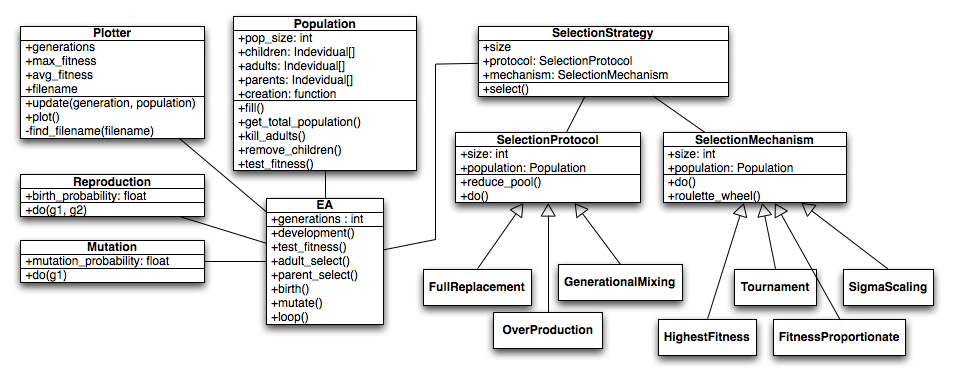
\includegraphics[width=\textwidth]{diagrams/classdiagram.png}
    \end{center}
    \label{fig:classdiagram}
    \caption[Class diagram]%
    {Class diagram for the basic EA. Not all subclasses and attributes of subclasses are included.}
\end{figure}

\subsection{Individual}
This is where the genotype, phenotype and fitness value gets stored. This class also have 
a method for calculating fitness value, based on a fitness function given as a parameter to
the constructor. You would normally inherit from this class in your EA.
The class also have an empty implementation of the function $create\_child$. This is used as an
abstract method. Subclasses should have their own implementation of the $create\_child$ method. \\


In the One-Max problem, this class gets extended to an BinaryVector class. This is a pretty shallow
extension. All it does is implement conversion between genotype and phenotype, create a randomly
chosen value representation and implement the $create\_child$ method.

\subsection{Population}
The Population class stores all information about all the individuals. It has separation for children and adults.
It also holds temporary information about the adults selected as parents. 

The population class has a method for looping through all individuals and calculate fitness using the individual's
fitness() method. If there's need for a free for all competition in the fitness testing (like in Colonel Blotto), the 
population class could be extended and the $test\_fitness()$ method can be overwritten. \\

The population class also holds a method for filling a population with individuals. This is used by sending a 
closure function as a constructor argument, and executing the $fill()$ method. A closure function is a function
storing values and returning a function that uses those stored values. This is used to make the filling of the
population as generic as possible. So typically, the returning function should return an instance of the Individual
class (or a subclass).

\subsection{Selection Strategy}
As seen in the \hyperref[fig:classdiagram]{class diagram}, the Selection Strategy consists of multiple classes
and subclasses. There are two classes in direct contact with the SelectionStrategy class; Protocol and Mechanism.
Those two classes, contain the implementation of the different protocols and mechanisms. Both have a similar
interface with the do method and a subclass for each different implementation.

In the do method, the population gets altered according to the rules specified by the protocol or strategy. The
main SelectionProtocol class, has a $reduce\_pool()$ method. This can be used by the protocols to reduce the 
population to a fitable size. I.e with ($\mu$, $\lambda$) and ($\mu + \lambda$) selection. \\

The mechanisms are slightly more complex than the protocols. With mechanisms using roulette wheel, the 
subclass need to override the probability function inherited from the base class. This method is used to find the
different "degree of sectors" on the roulette wheel. If the probability function uses aggregated values, such as
fitness sum, average fitness and so on, one could implement those in a $set\_values()$ method and set values
as object variables. Run the $set\_values()$ method in the $do()$ method. This way no unnecessary calculations
are performed. The mechanisms using roulette wheel should return the execution of the $roulette\_wheel()$
method.  \\

The SelectionStrategy class is an umbrella for protocols and mechanisms. Based on what constructor 
argument get's sent in. The arguments are one for protocol and one for mechanism. So if the FullReplacement
protocol is to be used, the argument will be a reference to that class. This way the strategy can include
a protocol and/or a mechanism. The abstraction also leads to insensitivity to the implementation of the protocols
or mechanisms. 

\subsection{Reproduction and Mutation}
\label{sec:repmut}
The mutation and reproduction classes are fairly similar to each other, and similar implementation as the 
selection strategies. Due to size limitation all subclasses of the reproduction and mutation base classes are not
shown in the \hyperref[fig:classdiagram]{class diagram}. There are implemented solutions for uniform,
two point and one point crossover. All of these have fairly similar interface. The only difference is in the 
constructor arguments. The constructor arguments set, optionally, the position of the splitting, and for
uniform crossover it sets the probability for selecting parents to cross from. 

The usage interface should be similar on all reproduction and mutation subclasses. The $do()$ method should
take two individual parents for reproduction and one individual child for mutation. 

The genetic crossover methods returns two newly created children by using the individuals $create_child()$ method.

\subsection{Execution file}
The execution file, $main.py$, ties all classes together and initiates the EA class. All instances and generic coding
So instances are made from plotter, population, selection strategy for adults, selection strategy for parents, reproduction
and mutation. These objects are passed into the EA constructor. The created EA object can now initiate the evolutionary
loop. \\

The execution file can create all the sub classes for the specific EA problem, or one could separate this code out to 
modules if the code gets to big. \\

To solve the One-Max problem, the main file creates a BinaryVector subclass (from Individual), sets the fitness
calculation function to be passed on the creation of the binary vector, and the closure function for generating 
individuals (used by the population class). \\

Further more, the main class has an interface, using the $argparse$ python module, for handling different values
on the parameters for the EA. Read more about configuring these below. 

\subsection{Configuring}
The application is made as a command line tool. This means that one could use flags to alter settings. Below there
is a complete list of the different flags available for the running of the One-Max Problem. 

\begin{enumerate}
	\item \textbf{-ps}: Defines the population size. \textit{Defaults to 100}
	\item \textbf{-g}: Defines number of generations. \textit{Defaults to 100}
	\item \textbf{-s}: Defines the geno size. \textit{Defaults to 40}
	\item \textbf{-m}: Defines the mutation probability. \textit{Defaults to 0.0}
	\item \textbf{-b}: Defines the reproduction probability. \textit{Defaults to 0.9}
	\item \textbf{-reproduction}: Defines the reproduction probability. \textit{Defaults to 0.9}
	\item \textbf{-o}: Defines the output name for generated plots. \textit{Defaults to onemax}
	\item \textbf{-noplott}: Defines is the data should be plottet or not. Overrides $-o$ flag. \textit{Defaults to do plotting}
	\item \textbf{-protocol}: Defines the selection protocol for adult selection. Must be the same name as the class. \textit{Defaults to FullReplacement}.
	\item \textbf{-mechanism}: Defines the selection mechanism for parent selection. Must be the same name as the class. \textit{Defaults to FitnessProportionate}.
	\item \textbf{-e}: Defines elitism. If e < 1, fraction is used. 0 equals none. \textit{Defaults to 0.05}.
	\item \textbf{-t}: Defines truncation. Is a fraction of the total population.  0 equals none. \textit{Defaults to 0.1}.

\end{enumerate}

\textit{Note: For the $-protocol$ and $-mechanism$ flags, the classes must be imported to the execution file.}

\subsubsection{Troubles with iPython and argparse}
As described in \hyperref[sec:thirdparty]{Third party \& Dependencies}, this application uses matplotlib and scipy 
for plotting data. As far as I found, the library are dependent on using the interactive extension to python; iPython.

As I found out after implementing plotting, the iPython flags and command line tool overrides the application flags 
and configuration. I could not find any solution to this problem, given the time limit. 


